\documentclass[letterpaper, 12pt]{article}
\usepackage[francais]{babel}

\usepackage{amsmath,amsfonts,amsthm,amssymb, graphicx,wasysym,multirow}
\usepackage[latin1]{inputenc}

\pagestyle{plain}

\setlength{\topmargin}{-2cm}
\setlength{\textheight}{23.5cm}
\setlength{\textwidth}{18cm}
\setlength{\oddsidemargin}{-1cm}
\setlength{\parindent}{0pt}

%\pdfoutput=1


\begin{document}


1016 * -- Let's say that $A$, $B$ and $C$ are integers. If the greatest common divisor of $A$ and $B$ is $1$, then it can be said that $A$ and $B$ are relatively prime. If $C$ divides $A\,-\,B$, we write $A\equiv B\,(\mathrm{mod}\,C)$. Which of these statements is the famous Fermat's theorem and is used for advanced algorithms?\\

a$)$ {\sl Given relatively prime integers $a$ and $b$, then $b^{a\,-\,1}\equiv1\,(\mathrm{mod}\,a)$.} \\
b$)$ {\sl Given a prime number $p$ and an integer $a$, and that $p$ and $a$ are relatively prime, then
$a^{p\,-\,1}\equiv1\,(\mathrm{mod}\,p)$.} \\
c$)$ {\sl Given a prime number $p$ and an integer $a$, and that $p$ and $a$ are relatively prime, then
$p^{a\,-\,1}\equiv1\,(\mathrm{mod}\,a)$.} \\
d$)$ {\sl Every odd number is prime.}\\

Answer: b$)$\\

Explanation: \\
Fermat's theorem is:
{\sl Given a prime number $p$ and an integer
$a$, and that $p$ and $a$ are relatively prime, then
$a^{p\,-\,1}\equiv1\,(\mathrm{mod}\,p)$.}
The correct answer is b$)$.\\

1017-- Fermat numbers are numbers of the form $F_n=2^{2^n}\,+\,1,
n=0,1,2,\ldots$ For example, for $n=2$,
$17=2^{2^2}\,+\,1$ is a Fermat number. What is the largest known Fermat prime number?\\

a$)$ $1000$ \\
b$)$ $2^{2^4}\,+\,1$ \\
c$)$ $2^{2^5}\,+\,1$ \\
d$)$ $2^{2^6}\,+\,1$\\

Answer: b$)$\\

Explanation: \\
The largest known prime Fermat number is $2^{2^4}\,+\,1$. Fermat
thought that all his numbers were prime. He was right for $F_0=3$,
$F_1=5$, $F_2=17$, $F_3=257$ and $F_4=65\,537$. However, Euler has
shown that Fermat's general statement was false, since
$2^{2^5}\,+\,1=2^{32}\,+\,1=4\,294\,967\,297=641\cdot6\,700\,417$.
We now know that numbers $F_5,F_6,\ldots,F_{24}$ can be factored.
The correct answer is b$)$.\\

1018-- Some numbers can be written as the sum of two squares. For example, $13=4\,+\,9=2^2\,+\,3^2$ is such a number. Which of these numbers can be written as the sum of two squares?

a$)$ $3$ \\
b$)$ $3^2\,\times\,7=63$\\
c$)$ $3^2\,\times\,7^2=441$ \\
d$)$ $3^2\,\times\,11^3=11\,979$\\

Answer: c$)$\\

Explanation: \\
We must use a result that Fermat came up with : {\sl An integer $n$
can be written as the sum of two squares if and only if each of its
prime factors of the form $4k\,+\,3$ has an even exponent in the
prime factorization of $n$.} The first three numbers of the form
$4k\,+\,3$ are $3=0\,+\,3=4(0)\,+\,3$, $7=4\,+\,3=4(1)\,+\,3$ and
$11=8\,+\,3=4(2)\,+\,3$. Only $441$ has even exponents in the prime
factors of the form $4k\,+\,3$ of its prime factorization
Therefore, the answer is c$)$.\\


1334-- Mathtown's city clock rings every hour. It rings once at 1
a.m. and at 1 p.m, twice at 2 a.m. and at 2 p.m., $\ldots$, and 12
times at noon and at midnight. Furthermore, it rings twice at each
$30^{\textrm{th}}$ minute of each hour (that is, at 1:30 a.m., 2:30
a.m., and so on) and three times at the $45^{\textrm{th}}$ minute
of each hour (that is, at 1:45, 2:45, and so on.). How many times does the clock ring in 24 hours?\\

Answer: 276\\

Explanation:\\
For every hour on the hour, the clock rings:
$1\,+\,2\,+\,3\,+\,4\,+\,5\,+\,6\,+\,7\,+\,8\,+\,9\,+\,10\,+\,11\,+\,12\,+\,1\,+\,2\,+\,3\,+\,4\,+\,5\,+\,6\,+\,7\,+\,8\,+\,9\,+\,10\,+\,11\,+\,12\,=\,156$
times.\\
For every half hour, it rings $2\times24=48$ times.\\
For every 45$^{\textrm{th}}$ minute of each hour, it rings $3\times24=72$ times.\\
In total, the clock rings $156\,+\,48\,+\,72=276$ times.\\
The correct answer is 276.\\


1335-- Before the discovery of Mount Kilimanjaro, what was Africa's highest summit?\\

Answer: Kilimanjaro\\

Explanation: \\
Even before its discovery, Mount Kilimanjaro was Africa's highest mountain!\\

1336-- What animal walks on fours legs in the morning, on two legs at noon, and on three at night.? (This is the Sphinx enigma.)\\

Answer: Man\\

Explanation: \\
At the beginning of his life, man walks on four legs, at noon, he is halfway through his life and walks on his two legs. At night, he is old and walks with a cane. The correct answer is man.\\

1337-- Roufi's mom has three children: Rafiki, Zazu and the third child.  What is the name of the third child?\\

Answer: Roufi\\

Explanation: \\
The third child is Roufi.\\

1338-- A man stands on a river side. He wants to fetch a 40\,\$ bill from the other side of the river. However, he cannot get there swimming because the river is full of alligators. Furthermore, he cannot build a a raft or a canoe because there are no trees around. How does the man make it?\\

a) He crosses the river by walking on the alligator's heads.\\
b) He asks his pet parrot to go fetch the bill.\\
c) He starts playing the flute to make all the alligators go to sleep.\\
d) It is impossible to do it.\\


Answer: d)\\

Explanation: \\
This situation is not probable because 40\,\$ bills don't exist! \\

1339-- You are in a room where the floor, the ceiling and every wall are entirely covered with mirrors. You close the door and you find out that its back is also covered with a mirror. How many reflections of yourself do you see?\\

a) 0\\
b) 1\\
c) 6\\
d) An infinite amount.\\

Answer: a)\\

Explanation: \\
Since the room is entirely covered with mirrors and the door is closed, it is completely dark. Reflections are not possible because there is no light in the room. Therefore, the answer is a).\\

1340-- Zazu poors lemonade into a glass that has a 255 ml capacity. She adds 2 ice cubes of 5 ml each, in such a way that the glass is just about to spill over. If Zazu doesn't drink her lemonade right away and the ice cubes melt, how many millimeters of liquid will spill out of the glass?\\

a) It is impossible to know.\\
b) 2 ml of liquid will spill out.\\
c) 10 ml of liquid will spill out.\\
d) No liquid will spill out.\\

Answer: d)\\

Explanation: \\
No liquid will spill out. When ice melts, it undergoes a transition phase, from solid to liquid. It turns out that water density is greater than ice density. The total volume of matter in the glass actually decreases! Thus, the answer is d).\\

1341-- In Canada, is it legal for a widow's wife to marry her husband's brother?\\
a) Yes.\\
b) No.\\
c) We cannot know.\\
d) Sometimes, it is possible, sometimes it is not.\\

Answer: b)\\

Explanation: \\
It is not only illegal, but also impossible for a widow's wife to marry her husband's brother. Indeed, if the man is a widow, it implies that his wife is dead! Therefore, the answer is b).\\

1342-- In a cycling race, Relly Fasste passes the second racer. What is Relly Fasste's new position?\\

a) First position.\\
b) Second position.\\
c) Third position.\\
d) Second to last position.\\

Answer: b)\\

Explanation: \\
If Relly Fasste passes the second racer, he becomes the second racer himself. The answer is b).\\

1343-- A water lily on a pond doubles in size every day. On the twentieth day, it covers half the surface of the pond. After how many days will the water lily entirely cover the pond?\\

a) 21\\
b) 30\\
c) 31\\
d) 40\\

Answer: a)\\

Explanation: \\
The water lily covers half the pond area on the twentieth day. Since it doubles in size everyday, it will cover the whole pond on the next day. The answer is a).\\

1344-- Two brothers possess the same amount of money. However, since
the eldest child is 10 years older than his brother, he thinks he
should have 10\,\$ more than his brother. What amount must the
youngest child give to his brother for this to happen?
(Only type in the number corresponding to the amount of money.)\\

Answer: 5\\

Explanation: \\
The youngest brother must give 5\,\$ \ to his brother.  \\
Assume that the 2 brothers have $n$\,\$ each. If the youngest brother gives 5\,\$
to his brother, he has ($n\,-\,5$)\,\$ left and his older brother now has ($n\,+\,5$)\,\$.
The difference of these two amounts is
$(n\,+\,5)-(n\,-\,5)=n\,+\,5\,-\,n\,+\,5=10$.  The answer is 5.\\

1345-- Voltaire's enigma\\
\begin{center}{What is of all things in the world,\\
The longest and the shortest,\\
The quickest and the slowest,\\
The most divisible and the most spread out,\\
The most neglected and the most regretted,\\
Without which no one can do anything,\\
That devours all that is small,\\
And invigorates all that is big?\\
Who am I?\\}
\end{center}

Answer: time\\

Explanation: \\
The answer to this enigma is time.  \\
Here is an explanation taken from the site:\\
http ://pages.globetrotter.net/pcbcr/zadig.html\\

The great wizard first proposed this question: \og What is of all
things in the world, the longest and the shortest, the quickest and
the slowest, the most divisible and the most spread out, the most
neglected and the most regretted, without which no one can do
anything, that devours all that is small,
and invigorates all that is big?\fg\\\

It was Itobad's time to speak. He answered that a man like him
didn't have anything to do with enigmas, and that it was enough to
have lived through swords and spears. Some people said that the
answer to the enigma was fortune, other people said the Earth,
others said light. Zadig said that it was time.\og Nothing is longer
than time, he said, because it is the measure of eternity, nothing
is shorter, because it's missing to all our projects, nothing is
slower for the one waiting, nothing is faster for the one enjoying
himself, it spreads out until infinity on a large scale, and divides
infinitely on a small scale, all men neglect it, while regretting
its loss, it makes us forget the things that are not worthy and it
immortalizes the important things.\fg\
The assembly decided that Zadig was right.\\


1346-- Voltaire's enigma\\
\begin{center}{What is it that we receive without thanking, \\
Which we enjoy without knowing how,\\
That we give to others while keeping it,\\
And that we lose without realizing it?\\
Who am I?\\}
\end{center}

Answer: life\\

Explanation: \\
The answer to this enigma is life.\\

1347-- How many times does the letter F appear in the following sentence?\\

{\Large\textbf FINISHED FILES ARE THE RE-\\
SULT OF YEARS OF SCIENTIF-\\
IC STUDY COMBINED WITH THE \\
EXPERIENCE OF YEARS}\\


Answer: 6\\

Explanation: \\
The letter F appears six times in this sentence. The brain doesn't actually process the word \og OF\fg. If you have answered 3, you are in the average. Very few people answer 6.\\
(Taken from the site : http ://www.e-monsite.com/samir/rubrique-1009354.html)\\

1348-- \begin{center}{Que j'aime \`a faire apprendre\\
un nombre utile aux sages\\
Immortel Archim\`ede, artiste, ing\'enieur\\
Qui de ton jugement peut priser la valeur?\\
Pour moi, ton principe eut de f\'econds avantages.\\}\end{center} This French poem gives the value of the number $\pi$ to 30 decimal places. What is it? (Hint: You don't need to know any French to answer.)\\

Answer: 3.141592653589793238462643383279\\

Explanation: \\
The number of letters for each word corresponds to the value of the numbers that make up the number $\Pi$ up to the 30th decimal place.\\

Que j'aime \`a faire apprendre: 314159\\
un nombre utile aux sages: 26535\\
Immortel Archim\`ede, artiste, ing\'enieur: 8979\\
Qui de ton jugement peut priser la valeur?: 32384626\\
Pour moi, ton principe eut de f\'econds avantages.: 43383279\\
(Taken from the site http ://www.e-monsite.com/samir/rubrique-1007309.html)\\


1349--\begin{center}{Que j'aime \`a faire apprendre un nombre utile aux
sages! \\
Glorieux Archim\`ede, artiste ing\'enieux,\\
Toi de qui Syracuse aime encore la gloire,\\
Soit ton nom conserv\'e par de savants grimoires! \\
Jadis, myst\'erieux, un probl\`eme bloquait \\
Tout l'admirable proc\'ed\'e, l'oeuvre grandiose\\
Que Pythagore d\'ecouvrit aux anciens Grecs. \\
O quadrature! vieux tourment de philosophe!\\
Insoluble rondeur, trop longtemps vous avez \\
D\'efi\'e Pythagore et ses imitateurs. \\
Comment int\'egrer l'espace plan circulaire?\\
Former un triangle auquel il \'equivaudra? \\
Nouvelle invention : Archim\`ede inscrira \\
Dedans un hexagone; appr\'eciera son aire \\
Fonction du rayon. Pas trop ne s'y tiendra :\\
D\'edoublera chaque \'el\'ement ant\'erieur; \\
Toujours de l'orbe calcul\'ee approchera;\\
D\'efinira limite; enfin, l'arc, le limiteur\\
De cet inqui\'etant cercle, ennemi trop rebelle!\\
Professeur, enseignez son probl\`eme avec z\`ele!...\\}
\end{center}
This French poem gives the value of the number $\pi$ to the 30th decimal place. What is it? (Hint : You don't need to know any French to answer.)\\

Answer: \\
3,141592653589793238462643383279502884197169399375105820974944592307816406286\\
208998628034825342117067982148086513282306647093844\\

Explanation: \\

The number of letters for each word corresponds to the value of the numbers that make up the number $\Pi$ to the 126th decimal place.\\


Que j'aime \`a faire apprendre un nombre utile aux sages! : 31415926535\\
Glorieux Archim\`ede, artiste ing\'enieux, : 8979\\
Toi de qui Syracuse aime encore la gloire, : 32384626\\
Soit ton nom conserv\'e par de savants grimoires! : 43383279\\
Jadis, myst\'erieux, un probl\`eme bloquait : 50288  (Noter qu'un mot de 10
lettres est remplac\'e par 0.)\\
Tout l'admirable proc\'ed\'e, l'oeuvre grandiose : 4197169\\
Que Pythagore d\'ecouvrit aux anciens Grecs. : 399375\\
O quadrature! vieux tourment de philosophe! : 105820\\
Insoluble rondeur, trop longtemps vous avez : 974944\\
D\'efi\'e Pythagore et ses imitateurs. : 59230\\
Comment int\'egrer l'espace plan circulaire? : 781640\\
Former un triangle auquel il \'equivaudra? : 628620\\
Nouvelle invention : Archim\`ede inscrira : 8998\\
Dedans un hexagone; appr\'eciera son aire : 628034\\
Fonction du rayon. Pas trop ne s'y tiendra : : 825342117\\
D\'edoublera chaque \'el\'ement ant\'erieur; : 0679\\
Toujours de l'orbe calcul\'ee approchera; : 821480\\
D\'efinira limite; enfin, l'arc, le limiteur : 8651328\\
De cet inqui\'etant cercle, ennemi trop rebelle! : 2306647\\
Professeur, enseignez son probl\`eme avec z\`ele!... : 093844\\

You can simply read off the numbers that make up $\Pi$ from top to bottom.\\

The answer is:\\
3.1415926535897932384626433832795028841971693993751058209749445\\
92307816406286208998628034825342117067982148086513282306647093844\\

1350-- Hy Kerr is hiking on Mount Ten. Some parts of his hike are very steep, so Hy Kerr progresses in a slower fashion in those parts. He gets to the summit by the end of the day. The next morning, Hy Kerr hikes back down. Since the way down is easier, it also takes less time to complete. If Hy Kerr had started his hike at the same time on each day, is there a point on the hike where he was on the ascent and on the descent at exactly the same time of the day?\\
a) Yes.\\
b) No.\\
c) It is impossible to know.\\
d) Who cares.\\

Answer: a)\\

Explanation: \\
Suppose that Hy Kerr has a twin brother that is doing the same hike as him, with the only difference being that he starts the ascent when Hy Kerr starts his descent. At some point on the way, they will cross. Thus, there exists a point on the hike where Hy Kerr was both at the same time of the day. However, we don't have enough information to know where this point is. The answer is a).\\

1351-- Obelix is visiting Asterix and decides to go back to his house that is 15 km away. He jumps on his bicycle and rides it at 15 km/h. At the same time, his dog Idefix, who was also at Asterixs' house, leaves with him. However, Idefix drank some magic potion and therefore is able to run at 18 km/h. He keeps doing laps between Obelix' and Asterix' house. How many kilometers did the little dog run before Obelix got to his house?\\

Answer: 18\\

Explanation: \\
Obelix had to ride 15 km. Since he is moving at 15 km/h, it takes him 1 hour to get home. During this time, Idefix is running at 18 km/h. He thus travels 18 km. The answer is 18.\\

1352-- A farmer possesses 25 cows who all die, but 5. How many cows does he have left?\\

Answer: 5\\

Explanation:\\
The statement says that 5 cows stay alive. The answer is thus 5.\\

1353-- The size of a water lily doubles everyday and it takes 24 days to entirely cover the pond where it is growing. How many days would 2 such water lilies take to entirely cover the same pond?\\

Answer: 24\\

Explanation: \\
On the 24$^{\textrm{th}}$ day, both water lilies are covering half the pond. Together, they cover the entire pond. The answer is 24.\\

1354-- When I am named, I don't exist anymore. Who am I?\\

Answer: silence\\

Explanation: \\
The answer to this enigma is silence.\\

1355--
A prisoner is standing in front of two doors identified by the letters A and B. One door leads to freedom, whereas the other door leads to an endless underground maze. The prisoner is guaranteed to die if he makes the wrong choice. A guardian is standing in front of each door. One of the guardian always lies, whereas the other one always tells the truth. The prisoner is allowed one single question. Which of theses choices would surely allow the prisoner to find his way to freedom?\\

a) Whatever question the prisoner asks, he will not be able to find the right door.\\
b) The prisoner asks one of the guards:\og If I were to ask your colleague if he tells the truth, what would he say?\fg This way, the prisoner can determine which door is the right one.\\
c) The prisoner asks one of the guards: \og If I ask your colleague if you are lying, what will he say?\fg. This way, the prisoner can determine which door is the right one.\\
d) The prisoner asks one the guards: \og If I ask your colleague which door leads to the exit, what will he answer?\fg . This way, the prisoner can determine which door is the right one.\\

Answer: d)\\

Explanation: \\
The prisoner must ask one of the guards:
\og If I ask your colleague which door leads to the exit, what will he answer?\fg \\
The two tables below show the possible outcomes of this question.
  \\


\begin{tabular}{|c|c|} \hline
{\bf Door A      }          & {\bf Door B}  \\ \hline \hline

Door leading to freedom.                 &  Door leading to death.
\\
\hline Door A's guard lies. & Door B's guard tells the truth. \\
\hline
Door B's guard tells the truth. &  Door A's guard lies. \\
\hline Door B's guard answers: Door A & Door A's guard answer: Door B\\
\hline Door A's guard answers: Door B:  & Door B's guard answers:
Door B\\ \hline


\multicolumn{2}{c}{}\\
\hline
{\bf Door A}                & {\bf Door B}  \\ \hline \hline

Door leading to death.                 & Door leading to freedom. \\
\hline
Door A's guard lies.      & Door B's guard tells the truth. \\
\hline  Door B's guard tells the truth.  & Door A's guard lies.
\\ \hline Door B's guard answers: Door B & Door A's guard answer: Door A\\ \hline Door A's guard answers: Door A & Door B's guard answer: Door A \\ \hline
\multicolumn{2}{c}{}\\
\end{tabular}

We notice that with this question, the prisoner has to choose the other door. In each case, it will lead him to freedom. The answer is d).\\

1356--  To get in to the hottest club in Math Town, besides being hip, one has to know the password. A first person walks to the doorman. The previous person having said 10, the person replies 3 and is allowed in to the club. A second person walks to the doorman and the doorman says 5. The customer replies 4 and is allowed in. A third person answers 4 again to the number 4 spoken out by the doorman and is also let in. Another club-goer walks up and replies 3 after the doorman had said the number 6. When the fifth person walks up to the doorman, the doorman had said the number 1. What must this person answer to be allowed in to the club?\\

Answer: 3\\

Explanation: \\
The word ten is made up of 3 letters. The appropriate answer to the
number 10 is thus 3. Similarly, the answer to five, four, and six
are respectively 4, 4, and 3. Since the word one is made up of three
letters, the appropriate answer is 3.
Therefore, the answer is 3.\\

1357--  My presence often shows absence. Bitten, I leave a bitter feeling. Who am I?\\

Answer: dust\\

Explanation: \\
The answer to this enigma is dust.\\
(Taken from the site http ://www.enigmathic.com/)\\

1358-- I start with an e, end with an e, and contain a single letter. Still, I am not the letter e. Who am I?\\

Answer: envelope\\

Explanation: \\
The answer to this enigma is an envelope.\\
(Taken from the site :  http ://www.enigmathic.com/)\\

1359-- Alive without breath, cold as death, never thirsty, always drinking, clad in a mail armor, but silent. Who am I?\\

Answer: fish\\

Explanation:\\
The answer to this enigma is fish.\\
(Taken from the site http ://www.enigmathic.com/)\\

1360--
A bowl contains one marble. The number of marbles in the bowl doubles every minute and is full after 60 minutes. How many minutes does it take to fill a bowl a quarter-full?\\

Answer: 58\\

Explanation: \\
It is easier to find the solution by starting at the end. When knowing that the bowl is full after 60 minutes. We can deduct that it is half-full after 59 minutes. Thus, we can conclude that the bowl is a quarter full after 58 minutes. The answer is 58.\\


1361-- A plane leaves Montreal for Vancouver and travels at 500 km/h. Another plane leaved Vancouver for Montreal and travels at 450 km/h. Which plane will be the closest to Vancouver when they meet?\\

a) The plane flying to Montreal.\\
b) The plane flying to Vancouver.\\
c) Both planes will be at the same distance from Vancouver.\\
d) It is impossible to know which plane will be the closest to Vancouver.\\

Answer: c)\\

Explanation: \\
Both planes will be at the same distance from Vancouver, because, when they meet, they are right next to each other.
This answer is c).\\



1362-- What has a hat, but no head, and a foot, but no shoe?\\

Answer: mushroom\\

Explanation: \\
The answer to this enigma is mushroom.\\
(Taken from the site http ://www.enigmathic.com/)\\



1363-- Five people are sitting in a circle in such a way that they can see the four other people. They are not allowed to talk or to make signs to the others. They know there are at least two yellow hats and two black hats. How many people can determine the color of their hat?\\

Answer: 2\\

Explanation: \\
Here is a drawing showing the setting of this problem:
    \begin{center}
    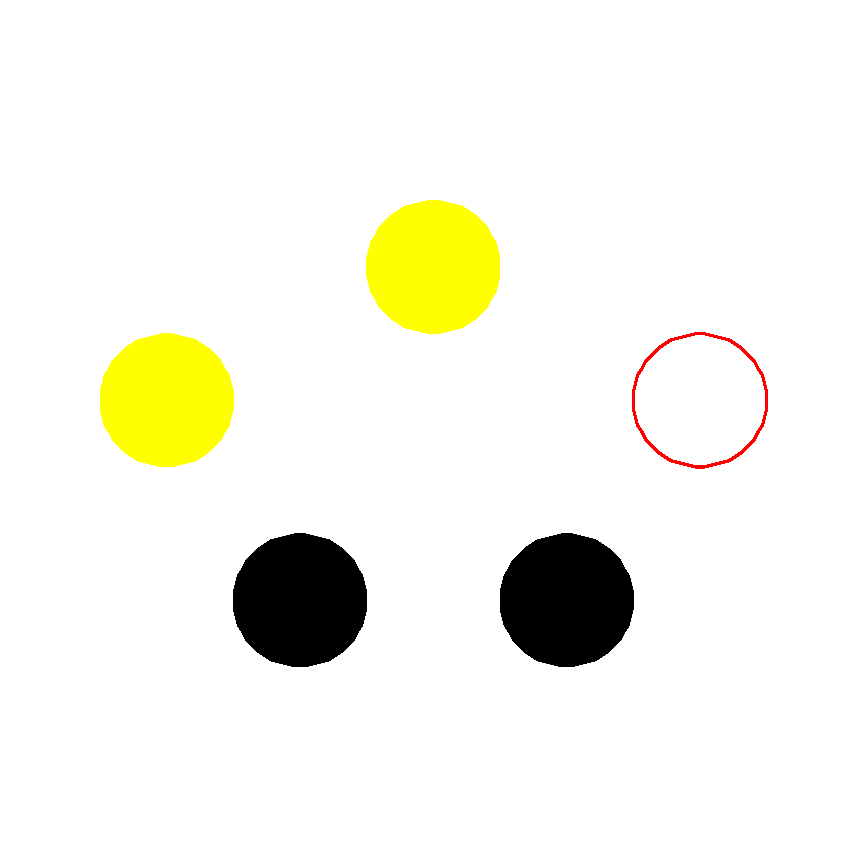
\includegraphics[width=6cm,bb=0 0 400 400]{chapeaux.eps}
% chapeaux.eps : 300dpi, width=3.39cm, height=3.39cm, bb=0 0 400 400
    \end{center}

Two people are wearing a yellow hat and two others are wearing a black hat. The color of the fifth hat is unknown. There are two cases.\\

Suppose that the unknown hat is yellow. The two people with a black hat see three people with a yellow hat. Thus, these two people can determine that they are wearing a black hat.\\

Now, suppose that the unknown hat is black. The two people with a yellow hat see three people with a black hat. Thus, these two people can determine that they are wearing a yellow hat.\\

In both cases, there are always two people that can determine the color of their hats. The answer is 2.\\

1364-- Five people are sitting in a circle, in such a way that they can see the four other people. They are not allowed to talk or to make signs to each other. Each person is wearing either a black or a yellow hat. They know there are at least 2 yellow hats and 2 black hats. When a person determines the color of their hat, he/she must say aloud : \og I know the color of my hat\fg. How many people can determine the color of their hats?\\

Answer: 5\\

Explanation: \\
Here is a drawing showing the setting of this problem :
    \begin{center}
    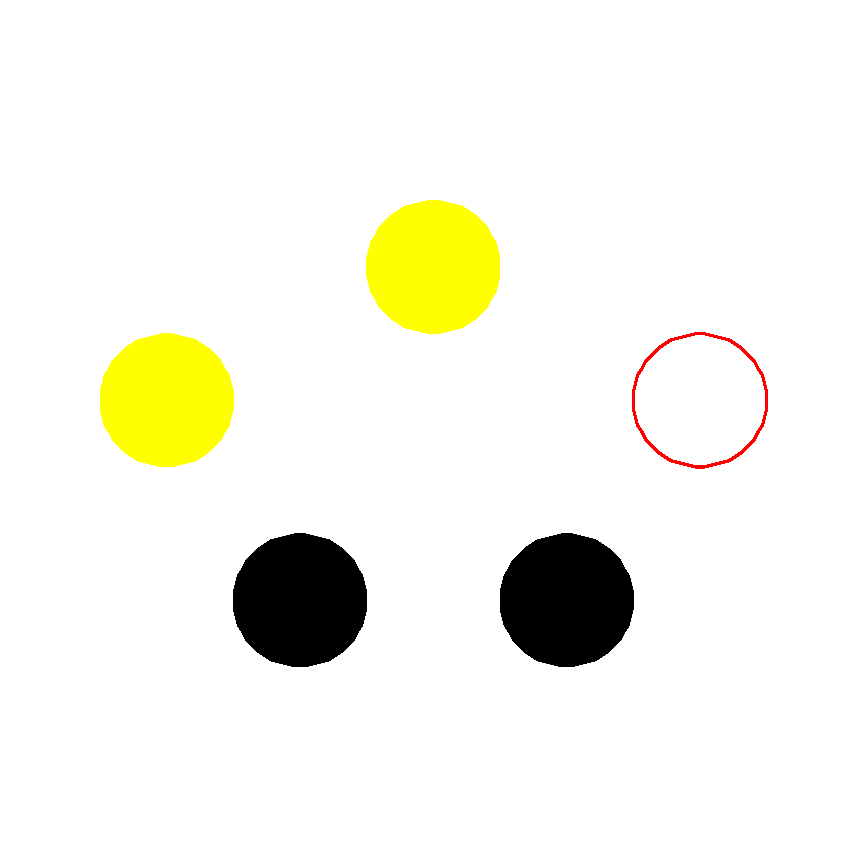
\includegraphics[width=6cm,bb=0 0 400 400]{chapeaux.eps}
% chapeaux.eps : 300dpi, width=3.39cm, height=3.39cm, bb=0 0 400 400
    \end{center}

Two people are wearing a yellow hat and two others are wearing a black hat. The color of the fifth hat is unknown. There are two cases. Suppose the unknown hat is yellow. The two people with a black hat both see three people with a yellow hat. They will both say : \og I know the color of my hat! \fg\ The three other people see two yellow hats and two black hats. Since two people have said : \og I know the color of my hat! \fg\ and these are the ones with the black hats, this indicates to the three silent people that they had seen three hats of the same color. Thus, the three remaining people can determine that they are wearing yellow hats. Therefore, all five people can determine the color of their hats.\\

The same logic applies to the other case. Suppose the unknown hat is black. The two people with a yellow hat both see three people with a black hat. They will both say : \og I know the color of my hat! \fg\ The three other people see two black hats and two yellow hats. Since two people have said : \og I know the color of my hat! \fg\ and these are the ones with the yellow hats, this indicates to the three silent people that they had seen three hats of the same color. Thus, the three remaining people can determine that they are wearing black hats. Therefore, all five people can determine the color of their hats.\\

In both cases, all five people can determine the color of their hats.\\

The answer is 5.\\


1365-- In a large company, 50 employees are working in the management department. Some of those employees are bilingual, some are not. If 2 employees are randomly chosen, at least one of them is bilingual. Which of these choices gives the right number of bilingual et unilingual employees?\\

a) 1 unilingual et 49 bilingals\\
b) 15 unilingual et 35 bilingals\\
c) 25 unilingual et 25 bilingals\\
d) 40 unilingual et 10 bilingals\\

Answer: a)\\

Explanation: \\
If there were 2 unilingual employees, it would be possible to pick them and form a pair of bilingual employees. The statement says that there is always at least one bilingual employee in each pair. Therefore, there can only be a single unilingual employee. The answer is a).\\


\end{document}
